\section{Implementazione}
Uno degli obiettivi principali del progetto \emph{PathS} è di fornire indicazioni di navigazione ai suoi utenti. Si è quindi presentata la necessità di dover rispondere a quesiti di \emph{routing} utilizzando le informazioni raccolte tramite le operazioni di campionamento e l'interrogazione del servizio di cartografia. 

Allo scopo di agevolare l'implementazione del componente e di ottimizare le operazioni di calcolo è stata selezionata per l'utilizzo la libreria \emph{PGRouting} la quale fornisce un grande supporto in questo senso. Questa estensione si appoggia alle funzioni \emph{GIS} del database introducendo le capacità di calcolo del percorso tramite l'utilizzo di molti algoritmi di flusso generici già implementati e configurabili ad esempio Floyd-Warshall, Shortest Path A*, Dijkstra e \emph{Traveling Sales Person}.

Tuttavia per poter operare correttamente la libreria necessita che siano  verificate alcune precondizioni sulla base dati da utilizzare, in particolare:
\begin{itemize}
	\item la rete di trasporto deve contenere informazioni corrette in corrispondenza delle intersezioni e degli estremi dei tratti adiacenti;
	\item la base dati deve contenere le informazioni sulla topologia della rete affinché si possa costruire un grafo utilizzabile dagli algoritmi.
\end{itemize}

Per affrontare il primo problema, la libreria mette a disposizione una funzione di `\emph{noding}''. Tale procedura riceve in input la tabella in cui sono contenuti i dati geografici e un valore di tolleranza, quindi rielabora le informazioni cercando di rimuovere situazioni non coerenti ad esempio:
\begin{itemize}
 \item intersezioni non gestite come il caso \emph{(1)} in figura \ref{fig:pgrouting-noding}. In alcuni casi i segmenti presenti nel database potrebbero intersecarsi senza però che sia presente il corrispondente punto di intersezione. In questa situazione le successive operazioni di \emph{routing} non sarebbero in grado di sfruttare l'intersezione come punto di svolta. La procedura consulta quindi le coordinate \emph{GIS} per individuare le possibili sovrapposizioni e in corrispondenza delle stesse crea dei vertici aggiuntivi spezzando i segmenti originari. La procedura mantiene traccia del numero e dell'ordine in cui vengono decomposti gli elementi originali.
 \item segmenti adiacenti con estremi che non coincidono come il caso \emph{(2)} in figura \ref{fig:pgrouting-noding}.
\end{itemize}

\begin{figure}[ht]
  \centering
  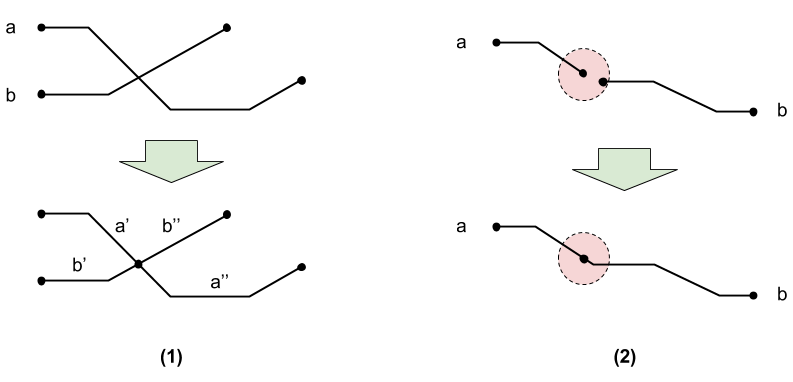
\includegraphics[width=.8\textwidth]{pgrouting-noding}
  \caption{\footnotesize{Casi in cui si applica la procedura di \emph{noding}.}}
  \label{fig:pgrouting-noding}
\end{figure}

L'applicazione della procedura di noding consente di ....

Si aggiungono le informazioni relative al grafo della rete di trasporto... 

Si è pronti ad utilizzare pgrouting pe ril calcolo dei percorsi. Il rislutato è un oggetto del tipo ... interpretato dal metodo della classe....

\section{Percorsi calcolati}
\subsection{Servizio Map Quest}
Interrogazione del servizio Map Quest come riscontro e \emph{fallback}. 
\subsection{Shortest Path}
Calcolo del percorso minimo con la libreria PGRouting.
\subsection{Percorsi con \emph{label}}
Calcolo dei percorsi valutando le label di luminosità e rumorosità. Viste e funzioni di supporto sul database. Modalità di calcolo dei costi, spiegazione delle formule.Requisiti del servizio di routing. Definizione del formato di colloquio (GeoJSON) e interpretazione lato client.